\ifx\wholebook\relax\else
\input{../Common.tex}
\input{../macroes.tex}
\begin{document}
\fi

\chapter{Tools to Understand Programs}\label{ch:loopvar}







\section{Tools for Understanding}
Now we present some practices to understand loops. Such pratices can be used in general to understand how your program work and they are useful to find errors.  For this purpose we will present you the Transcript, a small window to which messages can be written, and show how we can write message into it. The subsequent section will then use this functionality with loops.

\subsection{Transcript}
The \ct{Transcript}, with an uppercase letter, is a global variable
whose value is a small window in which output traces can be written as shown in Figure~\ref{fig:transcript}. A global variable is a variable that always exists, it had been defined once for all and that can be accessed from anywhere in the system. 

To open the \ct{Transcript} bring the World menu and select the menu item 'open', then select the menu item 'transcript', you should get the window
shown in Figure~\ref{fig:transcript}.  You also can pick
the transcript thumbnail like you made for the script editor or browser in the tools flap on the right and drop it into your desktop.

\begin{figure}[!htbp]
\centerline{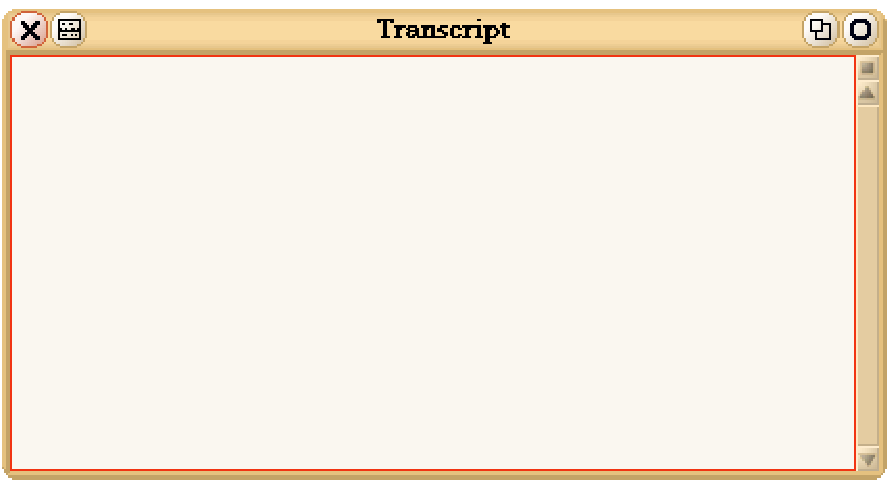
\includegraphics{Transcript}}
\caption{Here we have a Transcript}
\label{fig:transcript}
\end{figure}


\subsection{Using the Transcript}
We can send messages to the Transcript so that it
displays some texts. For example try the expression \ct{Transcript show: 'hello'}. It asks the Transcript to print the text 'hello'. More
precisely it asks the Transcript to display a string. 'hello' is a string composed by the characters \ct{\$h}, \ct{\$e}, \ct{\$l}, \ct{\$l} and \ct{\$o}. In \st a character is represented by the symbol \$ and the
character letter, but when we use \ct{''} we get a string composed of characters without needing to use \ct{\$}. 

The script~\ref{scr:transcript} presents a sequence of messages that we suggest you to try line by line. You will learn that the Transcript simply displays the strings one after the other ones and that we have to put space to be sure that the strings are not touching each other. If you want the Transcript to display the new text to the next line, you should tell it using the message \ct{cr}. Note that as we usually do not want to repeat Transcript in all the messages sent to it, we use a cascade to group messages as shown by the fourth line of the script~\ref{scr:transcript}.

The message \ct{show:} requires that you pass a string as argument, therefore if you want to print numbers you have to convert them into strings using the method \ct{printString}. \ct{12 printString} returns \ct{'12'} the string
that has the character \ct{\$1} as first element and character \ct{\$2} as second element. The expression \ct{Transcript show: 12 printString} displays the string '12' in the Transcript. Note that you can take several strings and turn them in a single one by sending the message \ct{,} to a string and passing the other as argument. The expression \ct{'Squeak',' is ', 'fun'} appends the three strings and returns the string \ct{'Squeak is fun'}.

\begin{scriptwithtitle}{Some expressions to write in the Transcript}\label{scr:transcript}
Transcript show: 'hello'.
Transcript show: ' on the same line'.
Transcript cr.
Transcript show: 'on another line it is better'; cr.
Transcript show: 'Squeak' , ' is ', 'fun' ;cr
\end{scriptwithtitle}


\begin{figure}[!htbp]
\centerline{\includegraphics{TranscriptWithHello}}
\caption{A trace in the Transcript showing the value of the variable \ct{length} at the beginning and the end of the loop.}
\label{fig:transcripthello}
\end{figure}


\begin{figure}[!htbp]
\centerline{\includegraphics{TranscriptWithValues}}
\caption{A trace in the Transcript showing the value of the variable \ct{length} at the beginning and the end of the loop.}
\label{fig:transcriptvalue}
\end{figure}



\subsection{Trace in Loops}
Using the Transcript functionalities we can now add trace generation to the
\scriptref{src:strangestair} as shown in the \scriptref{src:trace}. Executing now the script produces in the Transcript the trace shown in Figure~\ref{fig:transcriptvalue}.


\begin{scriptwithtitle}{Adding a trace to a script}\label{src:trace}
| caro length |
caro := Turtle new.
length := 10.
10 timesRepeat: [ Transcript show: '-start- length value is: ', 
                                                 length printString ; cr.
                caro go: length.
                caro turnLeft: 90.
                caro go: 5.
                caro turnRight: 90.
                length := length + 10.
                Transcript show: '-end- length value is: ', 
                                             length printString.
                Transcript cr]
\end{scriptwithtitle}

We suggest you to do the same with the scripts~\ref{src:strangestairtodo} and \ref{src:strangestairtodoby}.

\begin{scriptwithtitle}{Adding a trace to a script}\label{src:trace2}
| caro |
caro := Turtle new.
10 to: 100 by: 10  do: 
              [\bold{:length} | 
                 Transcript show: 'length: ', length printString; cr.
                 caro go: \bold{length}.
                 caro turnLeft: 90.
                 caro go: 5.
                 caro turnRight: 90]
\end{scriptwithtitle}




\subsection{Experimenting with Loops}\label{sec:transloops}
Now we want to show you that using the right message for loops can really simplify your programs and the way you solved them. Imagine that we want to generate lengths from 14 pixels to 100 pixels 2 by 2. You could write it using \timesRepeat the following way:

\begin{alltt}
| length |
length := 14.
43 timesRepeat: [ Transcript show: length printString ; cr.
                length := length + 2]
\end{alltt}

You may wonder where the 43 comes from. It comes from the following calculation 43 = 100 - 14 / 2. As you see this is not as
straightforward as the next solution to the problem using \ct{to:by:do:}

\begin{alltt}
14 to: 100 by: 2 do: [:length | Transcript show: length printString ; cr.]
\end{alltt}

The loop is executed until the specified upper limit is reached, the
limit itself included. For example, the following script produces 0, 3, 6, 9 and 12, while the following one only produces 0, 3, 6, 9 as 12 the next value is larger than the limit, 10, we specified.

 
\begin{alltt}
0 to: 12 by: 3 do: [:len| Transcript show: len printString;cr]
\end{alltt}

\begin{alltt}
0 to: 10 by: 3 do: [:length| Transcript show: length printString;cr]
\end{alltt}

As we mentioned earlier, \ct{to:do:} is equivalent to \ct{to:by:do:} the following scripts both produce 1, 2, 3, 4 and 5.

\begin{alltt}
1 to: 5 do: [:length | Transcript show: length printString ; cr.]
1 to: 5 by: 1 do: [:length | Transcript show: length printString ; cr.]
\end{alltt}

Note that with \ct{to:do:by:} you can also give negative numbers. The following script produces 4, 2, 0, -2 and -4.
\begin{alltt}
4 to: -4 by: -2 do: [:i | Transcript show: i printString ; cr.]
\end{alltt}








\summa

\begin{itemize}
\item The block passed to the message \ct{to:do:} and \ct{to:by:do:} require an argument. 

\item Block arguments are similar to method argument. \ct{[:length | ...]} is a block defining an argument named length. \ct{:length} is the argument name.  As blocks may have several arguments, \ct{|} ends the argument list.

\item Do not give name to a block argument the name of a variable already
existing in the script or method containing the block.

\end{itemize}
	






\ifx\wholebook\relax\else
\end{document}\fi
